\documentclass{article}[10pt]
\usepackage{scribe}
\usepackage{latexsym}
\usepackage{amsfonts}
\usepackage{algorithm}
\usepackage{algorithmic}
\usepackage{graphicx}
\usepackage{listings}

\setlength{\parindent}{0em}
\setlength{\parskip}{0.7em}

\newcommand{\Kdeletemin}{\texttt{delete-min}}
\newcommand{\Kinsert}{\texttt{insert}}
\newcommand{\Kdecreasekey}{\texttt{decrease-key}}

\title{Van Emde Boas Queues\\ 6.854 Scribe Notes \#4}
\date{September 15, 2003}
\author{Lecturer: David Karger\\ Scribes: Abhi Shelat (1999), Andrew  Menard (1999), Akshay Patil (2003), Daniel Myers(2006)}

\begin{document}

%%%%%%%%%%%%%%%%%%%%%%%%%%%%%%%%%%%%%%%%%%%%%%%%%%%%%%%%%%%%%%%%%%%%%
%%%%%%%%%%%%%%%%%%%%%%%%%%%%%%%%%%%%%%%%%%%%%%%%%%%%%%%%%%%%%%%%%%%%%%
% Your notes start here!
%%%%%%%%%%%%%%%%%%%%%%%%%%%%%%%%%%%%%%%%%%%%%%%%%%%%%%%%%%%%%%%%%%%%%%
%
% For theorems, lemmas, definitions, remarks, etc. use commands
% {\theorem{...}}, {\lemma{...}}, {\definition{...}}, etc.
% For proofs, use \begin{proof} ... \end{proof}
%
% For postscript figures (.ps) use the following block:
%
% \begin{figure}[h]
% \begin{center}
% \mbox{\psfig{figure=notes-nn-fig-mm.ps}}
% \caption{A very nice picture.}
% \label{fig:picture}
% \end{center}
% \end{figure}
%

% For encapsulated postscript figures (.eps) use the following block:
%  (also change documentstyle line )
% \begin{figure}[h]
% \begin{center}
% \mbox{\epsfbox{notes-nn-fig-mm.eps}}
% \caption{A very nice picture.}
% \label{fig:picture}
% \end{center}
% \end{figure}
%

%%%%%%%%%%%%%%%%%%%%%%%%%%%%%%%%%%%%%%%%%%%%%%%%%%%%%%%%%%%%%%%%%%%%%%

\section{Van Emde Boas Queues}
We would like to design a queue that only handles integers from
$0...C$, but supports all operations in $O(\log \log C)$ time.
This idea is first presented in ``Design and Implementation of an efficient
priority queue'', Mathematical Systems Theory 10 (1977).  Mikkel Thorup
provides some extensions in ``On RAM priority queues'' in SODA 1996.

This is a fantastic example of an efficient recursive data structure.
This structure also exploits the fact that keys in priority queues are 
most often integers and that computers have efficient operations for
manipulating the binary representations of integers (shifts, masks, logical
operations).  

Each vEB queue maintains the following information:

\begin{center}
\begin{tabular}{ll} 
Field & Notation \\ \hline
The current minimum & $Q.min$ \\ 
vEB queue on high halfword & $Q.summ$ \\
An array where each entry is a vEB queue on the low halfwords & $Q[x_h]$ \\ 
\end{tabular}
\end{center}
NB: 2006 lectures referred to $Q.summ$ as $Q.high$ and $Q[x_h]$ as
$Q.low$. It is also worthwhile to note that we 
store an element either in $Q.min$ or in $Q.summ$ and $Q[x_h]$, but 
not both.

Intuitively, we have the minimum item stored so we can
return it quickly. VEB priority queues
take the place of the buckets in the multi-level
bucket structure that was presented earlier (see Scribe Notes
2). Specifically, we note that the problem of finding the next minimum
among the buckets in the previous multi-level structure is actually a
priority queue problem, so we will recursively use our own priority
queue implementation to solve it!

There are $\sqrt{C}$ elements in the array ($Q[x_h]$ aka $Q.low$), and
each element in the array corresponds to a distinct high halfword
$x_h$.  (high halfword, $x_h$ = the higher-order $\frac{w}{2}$ bits in
the $w$-bit representation of a number, $x$; $w = \lg C$.  low
halfword, $x_l$ = the rest).  Thus when looking for an element, we can
look for the upper high halfword of the number, then recurse on the
low halfword

The purpose of the $summ$ is to quickly determine which low halfword vEB queues
actually contain elements.
If a low halfword vEB is non-empty, then we store
the vEB's address ($x_h$) in $Q.summ$.  Thus $Q.summ$ is a vEB of size $\sqrt{C}$
just like the low halfword vEBs as it stores $\frac{w}{2}$-bit numbers.

This is a rather straightforward approach and requires $O(C)$ space. (a more complex, randomized
approach is possible, leading to $O(\sqrt{C})$ space.)

\subsection{Inserts}

Consider the algorithm for inserting an element into the queue.

\begin{lstlisting}[mathescape]
Insert(x, Q):
  if Q.min = null:
    Q.min = x
    Return

  if Q.min > x:
    swap x, Q.min

  // divide x into its high halfword, x_h
  // and its low halfword, x_l
  (x_h, x_l) <- x 

  if Q[x_h].min = null:
    Insert(x_h, Q.summ)
    Q[x_h].min = x_l
  else:
    Insert(x_l, Q[x_h])
\end{lstlisting}

First we update all Q.min information in the first two if statements.

Then we split $x$ into halfwords.   This operation
can be done with a bit shift operation and a bitwise-AND operation.

At this point, we have split the problem of inserting $x$ into
this queue into a smaller problem of either inserting the high
halfword of $x$, or the low halfword of $x$.  If we have already
inserted $x_h$ in a previous operation, then it suffices to insert
$x_l$ in the low halfword queue that belongs to $x_h$.  If we have not
already seen $x_h$, then we need to insert it into our high halfword
queue.  However, this means that we can insert $x_l$ in $O(1)$ time
by simply changing $Q[x_h].min$.

The recursions finishes when the queues become small enough to
store as arrays (eg, 1-bit queues).

Notice that the function
makes only one recursive call to the {\sc Insert} function.  
Because all of the other operations are $O(1)$ time, the recurrence is
$$ T(b) = T(b/2) + O(1) $$
where $b$ is the number of bits in $x$.  Hence, $T(b) = O(\log b)$ and
since $b = \log C$, the algorithm runs in $O(\log \log C)$ time.

%% This image uses the randomized versoin of vEBs %%

%A sample queue with the elements $15, 3, 9$ would look like this:
\begin{figure}[h]
\begin{center}
  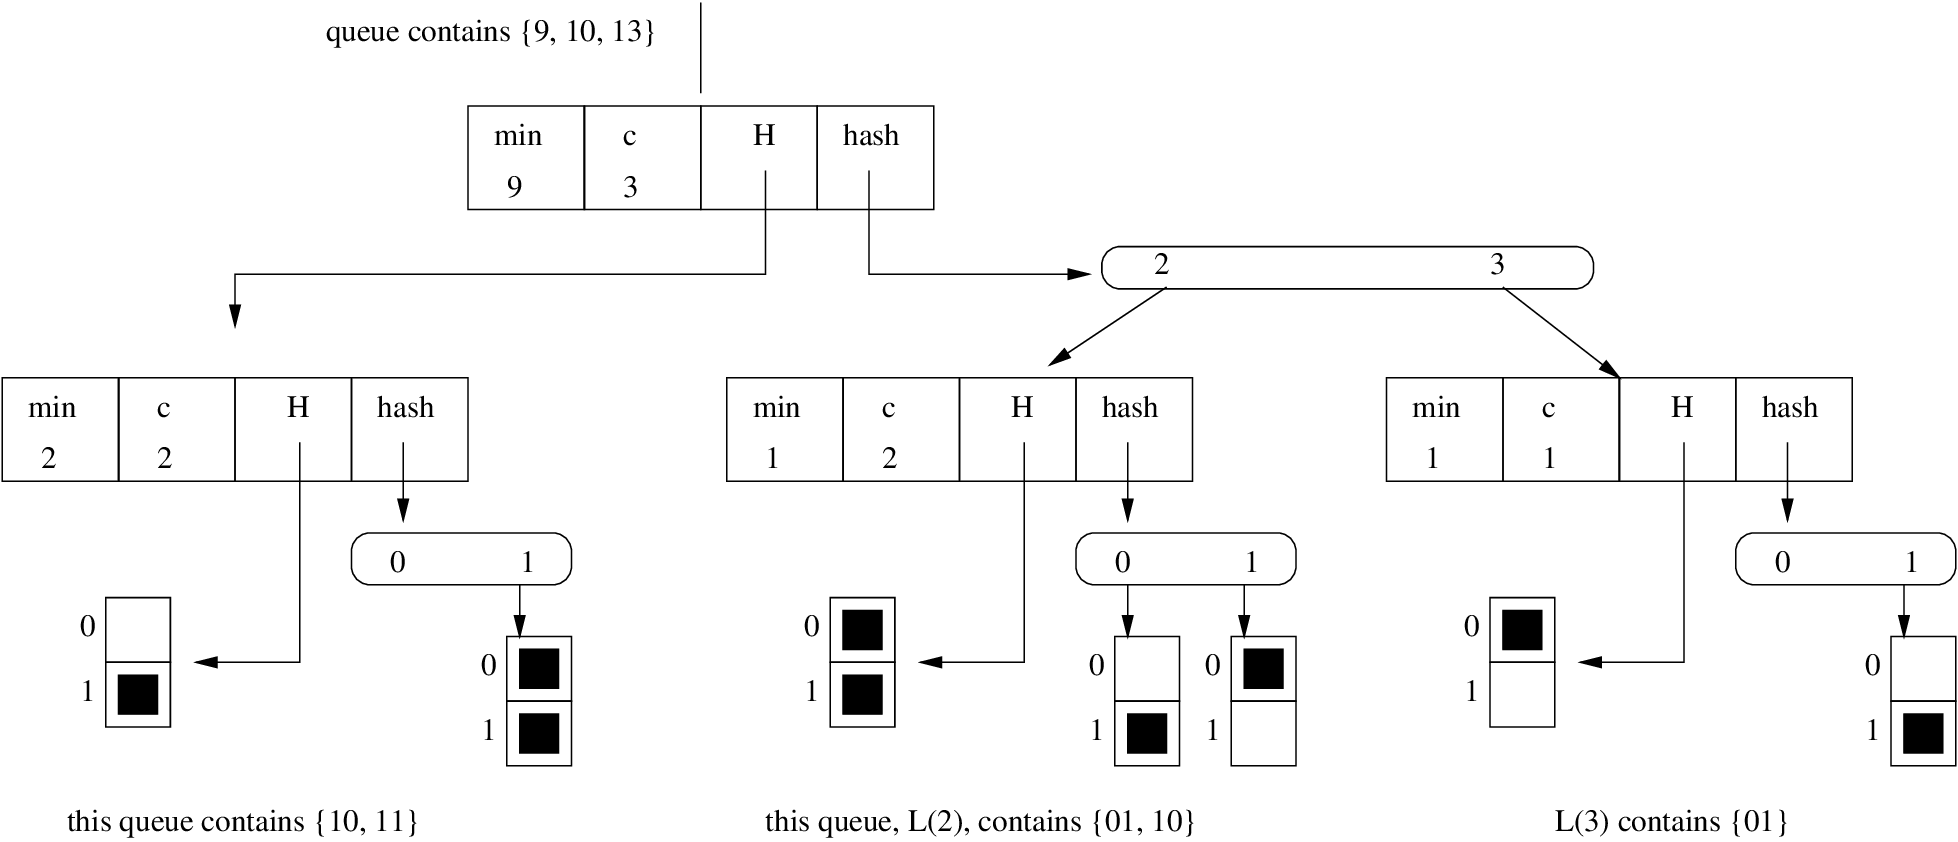
\includegraphics{veb.png}
\caption{A sample VEB queue.}
\label{fig:picture}
\end{center}
\end{figure}

\subsection{Find-Min}

Trivial, return Q.min.  This should take $O(1)$ time.

\subsection{Delete}

At somepoint, every element is a minimum element for some vEB.  We handle
this base case by deleting the min and then recalculating what the minimum
element is.  We must be mindful to keep $Q.summ$ up to date as well.
Otherwise, we merely drill down the levels of vEB until we reach our base case
situation.

\begin{lstlisting}[mathescape]
Delete(x, Q):
  if x < Q.min:
    Return 'Error x not in Q'

  if x = Q.min:
    first = Q.summ.min
    if first = null:
      Q.min = null
      Return

    // Create an element with high halfword 'first'
    // and low halfword 'Q[first.min]'
    Q.min = first | Q[first].min
    x = Q.min

  (x_h, x_l) <- x 
  Delete(x_l, Q[x_h])

  if Q[x_h].min = null then:
    Delete(x_h, Q.summ)
\end{lstlisting}

Once again, the running time for this algorithm is $O(\log \log C)$.
The reason why this again results in only one call to a $O(\sqrt{U})$ problem
is that even if {\sc Delete} is called twice, the second call implies that
the first call took only constant time. (if $Q(x_h)$ is now empty, that means
that the earlier call to {\sc Delete} was deleting that vEBs minimum, and only,
element. Such a call takes constant time, so we can now use our $O(\sqrt{U})$
time on updating $Q.summ$).

% Section on Queue Creation is removed because it was not covered in class
% and because it is irrelevant if we allow for O(U) space.


\subsection{Other supported operations}

Note that it is easy to support all of the following
operations in $O(\log \log C)$ time
\begin{itemize}
\item {\sc Max}$()$. Symmetric to the min.
\item {\sc Find}$(x)$. Determines whether the element exists in the queue.
\item {\sc Succ}$(x)$. Finds the smallest value in the queue that is 
                larger than $x$.  Returns nothing if $x$ is the largest.
\item {\sc Pred}$(x)$. Finds the largest value in the queue that is 
                smaller than $x$.  Returns nothing if $x$ is the smallest.
\item {\sc Delete-Min}$(x)$. Special case of {\sc Delete}.
\item {\sc Delete-Max}$()$. Removes the max element from the queue.  Works in the same way that {\sc Delete-Min} works.
\end{itemize}


\end{document}


